\documentclass[11pt,letterpaper]{article}
\usepackage{emnlp2017}
\usepackage{times}
\usepackage{latexsym}
\usepackage{url}

\usepackage{comment}
\usepackage{graphicx}
\usepackage{amsmath}
\usepackage{multirow}
\usepackage{enumitem}
\usepackage{amssymb}
\usepackage{tikz}
\usepackage{pgfplots}
\setlist[enumerate]{itemsep=0mm}
%\usepackage[utf8]{inputenc}
%\usepackage{acl2017}
%\usepackage{times}
%\usepackage{latexsym}
%\usepackage{url}

%\documentclass[11pt]{article}
%\usepackage{acl2016}
%\usepackage{times}
%\usepackage{url}
%\usepackage{latexsym}
%\usepackage{hyperref}
%\usepackage[tight,footnotesize]{subfigure}
%\usepackage{placeins}
%\usepackage{stfloats}
%\usepackage{helvet}
%\usepackage{courier}
\usepackage{color}
%\usepackage{multirow}
%\usepackage{booktabs}
%\usepackage{graphicx}
%\usepackage{caption}
%\usepackage{subcaption}
\graphicspath{ {figures/} }


%\usepackage[export]{adjustbox}

%\usepackage{array}
%\usepackage{tikz}

% Uncomment this line for the final submission:
\emnlpfinalcopy

%  Enter the EMNLP Paper ID here:
\def\emnlppaperid{792}

%\setlength\titlebox{5cm}
% You can expand the titlebox if you need extra space
% to show all the authors. Please do not make the titlebox
% smaller than 5cm (the original size); we will check this
% in the camera-ready version and ask you to change it back.


\newcommand*\textfrac[2]{
  \frac{\text{#1}}{\text{#2}}
}
\newcommand\BibTeX{B{\sc ib}\TeX}
\newcommand{\FIXME}[1]{\textcolor{red}{#1}}
\newcommand{\secref}[1]{Section~\ref{#1}} % section
\newcommand{\tabref}[1]{Table~\ref{#1}} % table
\newcommand{\figref}[1]{Figure~\ref{#1}} % figure
%\newcommand{\eqref}[1]{Equation~\ref{#1}} % equation
\newcommand{\mysubsection}[1]{\vspace{0.3em}\noindent\textbf{#1}}
\renewcommand{\baselinestretch}{0.955}
%\pgfplotsset{compat=1.13}

\title{Demographic-Aware Word Associations}

\author{Aparna Garimella, Carmen Banea, and Rada Mihalcea \\
  University of Michigan\\Ann Arbor, MI \\
  {\tt \{gaparna,carmennb,mihalcea\}@umich.edu}}

\date{April 2017}

\begin{document}
\maketitle

\begin{comment}
\FIXME{Pending tasks\\
Aparna: finalize LSA-based experiments (generic and demographics-aware) - 300 latent features\\
Aparna: update evals table (link to current results \url{https://docs.google.com/spreadsheets/d/1_i68_wBFhjXexa_yeo1xNA_BoBUUeMYLwlw_EXaThpM/edit#gid=1403989193})\\

NOTE: In terms of embeddings, the quarter data is already too small, and we see significant drops between using the culture or gender dataset on one side and using the quarter dataset on the other. In addition, for quarter data there are embeddings that simply don't return anything, as they are out-of-vocabulary. So even if we encounter a couple of occurrences in the data, it is not sufficient to generalize embeddings. Further more, the embeddings that I trained exist in a mixed space (with generic words and gender tagged words); the embeddings decisions are refined over both sides of a complementary demographic, so it would be unfair to compare it with generic embeddings versions that have access to only half the data (as the small quarters data set would do).}
\end{comment}

\begin{abstract}
 
Variations of word associations across different groups of people can provide insights into people's psychologies and their world views. To capture these variations, we introduce the task of demographic-aware word associations. We build a new gold standard dataset consisting of word association responses for approximately 300 stimulus words, collected from more than 800 respondents of different gender (male/female) and from different locations (India/United States), and show that there are significant variations in the word associations made by these groups. We also introduce a new demographic-aware word association model based on a neural net skip-gram architecture, and show how computational methods for measuring word associations that specifically account for writer demographics can outperform generic methods that are agnostic to such information.
  
  
%  Variations of word associations across different groups of people have been of interest to psychologists and linguists as they convey information about their psychologies. In this paper, we look at this variation in word associations over two demographics, namely gender and nationality. Based on the Mechanical Turk (MT) responses from males and females belonging to India and United States for a set of stimulus words, we show that associations indeed vary with gender and nationality. Using personal writings of people in the form of blog posts, we see if demographic information of people can improve word association prediction systems in comparison to the MT gold standard.
\end{abstract}



\section{Introduction}

%``Objects once experienced together tend to be associated in the imagination, so that when any one of them is thought of, the others are likely to be thought of also, in the same order of sequence or coexistence as before \cite{James90}."
%Hypothesis -- word associations vary with demographics; demographic information can help better predict people's associations.
%Considering nationality and gender as demographics (age? -- we do not have age information)

Understanding the associations that are formed in the mind is paramount to understanding the way humans acquire language throughout a lifetime of learning \cite{Elman1997,Rogers2004}. Furthermore, word associations are believed to mirror the mental model of the conceptual connections in a human mind, and constitute a direct path to assessing one's semantic knowledge \cite{Nelson2004,Mollin2009}. %Psycholinguistic studies focused on word associations have been conducted since early 1900s, and the field is actively pursued in Psychology, with the latest publication we are aware of describing a spiking neuron model of word association \cite{Kajic2017}.

Word associations start forming early in life, as language is acquired and one learns based on the environment where concepts lie in relation to each other. For example, we may learn to associate ``mother'' with ``warmth,'' or ``fire'' with ``burn.'' Yet, this mental model is not static but highly dynamic, and is shaped by new experiences over a lifetime.  For instance, \cite{Tresselt64} showed that word associations change with time, and that for respondents in younger age groups their variability is lower, % and the degree of association is higher, 
while for those in older age groups the variability is higher, as their life experiences modify the commonality between respondents from the same group. %% ARE WE MAKING AN ARGUMENT THAT GENERIC WORD ASSOCIATIONS WERE FINE IN THE EARLY 20 CENTURY, BUT ARE NOT FINE ANYMORE? I AM NOT SURE WE HAVE SUPPORT FOR THAT. I B ELIEVE TRESSELT REFERED TO CHANGES OVER THE LIFE OF AN INDIVIDUAL, NOT IN ABSOLUTE CHANGES OVER CENTURIES.
%CB: Tresselt did not study individuals over their lifetime, but conducted surveys at the same point in time for people meeting various demographic criteria.
%In the 1900s, the population was significantly more homogeneous and exposed to similar environments while having limited means of traveling and communication, thus triggering a high commonality between individuals of the same nationality. Nowadays, this is no longer the case, and generic word associations are no longer satisfactory. One option is to attempt to model such associations through the demographic attributes of the people from a given group. 

Computational linguistics has traditionally taken the ``one-size-fits-all" approach, with most  models being agnostic to the language of the speakers behind the language. With the introduction and adoption of Web 2.0, there has been an exponential increase in the availability of digital user-centric data in the form of blogs, microblogs and other forms of online participation. Such data often times can be augmented with demographic or other user-focused attributes, whether these are user-provided (e.g., from a user's online profile) or labeled using an automatic system. This enables computational linguists to go beyond generic corpus-based metrics of word associations, and attempt to extract associations that pertain to given demographic groups that would not have been possible without administering time consuming and resource intensive word association surveys.

While current NLP methods generally deal with more advanced tasks (relation extraction, text similarity, etc.), at their very core many of these tasks assume some way of drawing connections (or associations) between words. Therefore, as a step toward demographic-aware NLP, we choose to work on the core task of ``word association.'' The algorithms we introduce can be immediately applied to demographic-aware word similarity, and with some minor changes to demographic-aware text similarity. Future stages could also include demographic-aware labeled associations, and more advanced applications such as information retrieval (which relies heavily on word associations/similarity), demographic-aware keyword extraction, dialogue personalization, and so forth. Note that a few other researchers have explored demographic-aware NLP models with promising results, primarily focusing on the use of demographics for various forms of text classification \cite{Hovy2015} or sentiment and subjectivity classification \cite{Volkova2013}.



The paper makes several main contributions. 
%First, we create a novel dataset of demographic-aware word associations, consisting of approximately 300 stimulus words along with 800 responses per word collected from  a demographically-diverse group of respondents, for a total of 228,800 responses. 
First, we create a novel dataset of demographic-aware word associations, consisting of approximately 300 stimulus words along with 800 responses per word collected from  a demographically-diverse group of respondents, for a total of 228,800 responses.
% NEW -- APARNA
Removing spam responses resulted in 176,097 responses.
% END NEW -- APARNA
Analyses that we perform on this dataset demonstrate that indeed word associations vary across user dimensions.\footnote{This work is not centered around comparing different word forms, as one would encounter for example in British English and American English, but rather around different word associations that people with a particular demographic characteristic are inclined to make, 
%As such, we are not analyzing the usage of ``trousers'' vs ``pants,'' 
e.g., ``health'' in India is more strongly associated with ``wealth'', while in the United States it is more strongly associated with ``sick.''} 
% NEW -- APARNA
Second, we show that the associations we obtained follow the same pattern as those elicited during traditional classroom surveys. Third, we propose an evaluation metric suited for the free association norms task. Fourth, we introduce a demographic-aware model based on a skip-gram architecture and through several comparative experiments, we show that we are able to surpass the performance attainable on demographic agnostic models. %computational word association methods that account for user demographics outperform the performance of generic counterparts. % The main contributions of this work are: (1) creating a  new dataset with demographic-aware word associations, along with several analyses of variation across demographics and (2) conducting experiments and evaluations with four computational measures for demographic-aware word associations, including two traditional measures (MI and LSA) that are trained on data with known demographics, a recently introduced measure for specialized word embeddings \cite{Bamman2014}, as well as a novel embeddings model we introduce in this paper.

  %Depending on results, we can place more emphasis on our method
  %TODo maybe add some motivation why word associations are important and how they could be harnessed in NLP settings

%In this work, we first focus on creating a demographics-enhanced word association data set. To accomplish this goal, we focus on approximately 300 core English words for which we collect responses via the Mechanical Turk platform, as well as survey the respondents using a set of demographic questions.  We then seek to compare the results obtained in this study along the culture and gender dimensions with those automatically predicted using both traditional and novel approaches to derive word associations from large corpora enhanced with gender and culture information. 
%We hypothesize that word associations vary across demographics, and demographic knowledge about people can help better predict their associations for a given set of stimulus words.


%Specifically, given a word $W$, we process thousands of blog posts written by male and female bloggers belonging to India and United States and use their gender and nationality information to predict associations for it. 
%We use mutual information, latent semantic indexing (LSI), and word embeddings to estimate the association responses given demographic-labeled corpora in the form of blog posts.
%We conduct two sets of experiments, one with the demographic information for the blog posts, and second without this information.

We specifically focus on two demographic dimensions: location and gender. For location, we consider India and United States (US), choice made primarily because these two countries have a large English-speaking population, represented both on social media and on crowdsourcing platforms. %for several reasons, (1) each one of the countries has a large population, and has many online content authors who blog in English, (2) the countries possess a sufficient number of Amazon Mechanical Turk (AMT) workers to collect a robust gold standard from. In terms of gender, we consider male and female writings.



\section{Related Work}
Word associations have captured the attention of psychologists since at least the early 1900. In \shortcite{Kent10}, Kent and Rosanoff proposed the use of a set of 100 emotionally neutral words for word associations surveys. %The same year marked the beginning of a long term study conducted at the University of Minnesota focused on capturing the primary responses of students to trigger words, collecting data in 1910, 1927, 1933, 1952 and 1960 \cite{Jenkins1965}. The researchers have noticed that student's answers systematically changed across the datasets collected at different points in time, with the norms collected in a closer time frame displaying a higher correlation than those gathered between more distant survey dates. Also, primary responses that had a higher frequency exhibited a stronger resilience across data sets, while the usage of superordinate norms (e.g. a word whose meaning encapsulates the meaning of other words, such as blue representing the superset of teal, turquoise and navy) had steadily declined. While this study was surveying the same age group (students) at different points in time, \cite{Tresselt64} surveyed 738 subjects with ages ranging between 18 and 87, with particular care to include people from different socioeconomic classes (from unskilled laborers to professionals). Their conclusion was that primary responses' variability increases with age, as the strength of individuals' commonality decreases. For example, older people associated ``sleep'' with ``awake,'' instead of ``bed'' or ``dream'' which were the preferred answers of the younger age group. 
A psycholinguistics study that looked at the impact that the nationality of respondents may have on formed word associations was carried out by Rosenzweig \shortcite{Rosenzweig1961}, employing the stimulus word list proposed by Kent and Rosanoff \shortcite{Kent10} manually translated into several West European languages. Based on the primary responses coming from native speakers of English%(1008)
, French%(288)
, German %(331)
and Italian, %(229)
which were mapped back into English, the author concludes that the associations formed by speakers of the four languages are very similar, with ``almost half the comparisons in any pair of languages yielding agreements,'' where the most frequent responses are encountered across pairs of languages. % while rare responses do not correspond.  %Rosenzweig also mentions that the primary responses across genders of the same nationality have a high agreement, with French nationals split by gender agreeing 75\% of the time, while American nationals agreeing 82\% of the time. 
Given that the primary responses were compared across languages and people with a relatively common origin (West European), our work seeks to investigate whether similar results are encountered when looking at different locations (namely US versus India). Furthermore, our study is conducted in English from the beginning, to eliminate a third party's subjectivity in mapping primary responses from one language to another. %In addition, we want to verify whether the same high level of agreement holds between American men and women, and Indian men and women, while also exploring cross-cultural strength of word association between women and men.

%Given the change in associations over time,
%and the potential impact on such associations caused by other demographic factors, 
There have also been attempts in computational linguistics to derive associations not based on survey results (which are static and resource intensive), but based on statistics derived from large corpora \cite{Church89,Wettler89,Church90}. Research in semantic similarity can also be used to model associations based on several directions: (1) co-occurrence metrics that rely on large corpora such as PMI \cite{Church90}, second order PMI \cite{Islam2008}, or Dice \cite{Dice1945}; (2) distributional similarity-based measures, that characterize a word by its surrounding context such as LSA \cite{Landauer1997}, ESA \cite{Gabrilovich2007}, or SSA \cite{Hassan2011}; and  (3) knowledge-based metrics that rely on resources such as lexica or thesauri \cite{Leacock1998,Lesk1986,Jarmasz2003,Hughes2007}. However, most of these metrics have so far been applied to model the relatedness between two words, namely given a word pair, to score how similar the two words are; as such, they have not been used to predict free association norms, namely given a word, to attempt to determine the most likely word that a human would associate with that stimulus. 

%and metrics derived from large corpora, where the relative frequencies of pairs of words are seen as a measure of their association strength, and several corpus-based methods were developed to automate the association prediction: PMI \cite{Church89,Wettler89,Church90}. \FIXME{Expand on this}

Large word association databases exist, such as the one collected by Deyne et al. \shortcite{DeDeyne2013}, who used a set of 12,000 stimulus words and surveyed 70,000 participants. Yet to our knowledge, no concerted attempt has been made to gather word associations jointly with the demographic characteristics of the people behind them.

While not directly seeking to extract word associations but rather trying to represent language meaning through a locality lens, \cite{Bamman2014} have proposed using distributed representations to model words employed by social media users from different US states. They were able to show that the regional meaning of words can successfully be carried by word embeddings, for example the word ``wicked'' was most similar to the word ``evil'' in Kansas, while in Massachusetts, it was most similar to ``super'' (based on the cosine similarity of the words' vectorial representation). In contrast, our rationale in this article is to explore if word associations can be automatically derived from large corpora annotated with user-centered attributes such as location or gender. 



%One of the earliest works in word associations was conducted by Galton \shortcite{Galton79}, who asked human subjects to respond to a stimulus word with the first word that comes to their mind.
%There has been a large body of research in word associations in fields such as psychology and linguistics \cite{Clark70,Meara83,Isen85}, most of which involves human subjects and associations are predicted based on their most frequent response.
%Is the study below a psycholinguistic study or computational linguistics? If the latter, we should move it higher.
%Tresselt and Mayzner \shortcite{Tresselt64} have looked at the variation of word associations across %various age groups.
%They found that the variability in responses increases with age along with a decrease in the strength of communality.

\section{Word Associations Dataset}
Word association data collection typically consists of providing  participants with a list of words, also known in the psycholinguistics literature as {\it stimulus words}, and asking them to provide the first word that comes to mind in response to each stimulus. For instance, given a stimulus word such as {\it cat}, one would expect answers such as {\it dog} or {\it mouse}. Earlier work on word associations administered the tests in classroom settings, with 100 words per survey, and the results were compiled into tables of norms of word associations \cite{Kent10,Nelson2004}. 

Since our goal is to explore the effect of demographics on word associations, we created a task on Amazon Mechanical Turk (AMT) able to reach a wide and demographically diverse audience. The survey was structured into two sections: the word association part, followed by a demographic survey.
%, which all participants had to complete in order for their answer to be registered. 
Given the online nature of the survey, and since we aimed for a high quality dataset, each participant was presented with a set of 50 stimulus words at a time (instead of 100). The demographic section consisted of seven questions covering gender, age, location, occupation, ethnicity, education, and income.

\paragraph{Stimuli.} The stimulus list consists of a set of approximately 300 words. Among these,  99 words are sourced from the word list proposed by Kent and Rosanoff \shortcite{Kent10} (\textit{standard} list).\footnote{Note that this list originally included 100 words. The word ``foot'' was however misspelled in our survey, and instead we gathered answers for ``food.''}  The remaining words are identified using the method for finding word-usage differences between two groups introduced in \cite{Garimella16}, which relies on large collections of texts authored by the two groups to identify words that can be accurately classified by an automatic classifier as belonging to one group versus another. Using their method, we obtain 100 words as the top most different words between US and India (\textit{culture} list), and another set of 100 words as the top most different words between male and female (\textit{gender} list). 
%identified by \cite{Garimella16} in a cross-cultural experiment on word usage differences; and 100 words are obtained using a methodology for finding word-usage differences between groups similar to \cite{Garimella16}, but applied on gender data. Very briefly, their method  on identifying word usage differences between groups, but  from prior nationality experiments we conducted (Anonymous) for India versus US (\textit{culture} word list), and 100 by employing the same method, yet this time applied to gender (\textit{gender} word list). Specifically, each of these latter two lists are composed of the top 100 words emerging from experiments for each demographic dimension, such that they have the highest Adaboost accuracies over the baselines. (\FIXME{Maybe this needs to be clarified a little bit more.}) 
The reunion of these three lists results in 286 stimulus words for which we collect word associations. Examples are shown in Table \ref{tab:topResponses}.
%, and form a \textit{culture} word list and a \textit{gender} word list, respectively. Upon intersecting the three lists, we have 286 stimulus words that we surveyed for. 

\paragraph{Responses.} The task was published separately for respondents from US and India, as AMT has an option of only presenting the survey to people from a preselected geographical location. Six different surveys, each including approximately 50 stimulus words, were administered for each region. The survey was conducted in English for both countries, noting that one of the official languages of India is English (alongside Hindi). Each survey also included four spam-checking questions with previously known answers (e.g., {\it What is the color of the sky?}, with five options {\it blue}, {\it red}, {\it pink}, {\it green}, {\it yellow}), which were used to filter out respondents who were filling out the survey without reading the questions. 

For each set, we gathered 400 responses per region, resulting in 800 responses for both US and India. After removing the respondents who did not pass the spam-checking questions, we were left with an average of 752 responses per word, which we then balanced by gender, to retain an equal number of Indian women, Indian men, US women, and US men.
%. Since AMT does not allow us to filter respondents based on their gender, the male and female responses were not balanced in the resulting set. As such, to avoid any bias caused by including more responses from a given demographic, we randomly selected the respondents to each survey so as to retain an equal number of Indian women, Indian men, US women, and US men.
This resulted in 492 and 480 responses for the two sets of 50 \textit{standard} stimulus words, 436 and 468 for the \textit{culture} words, and 440 and 432 for the \textit{gender} words. Similar to \cite{Rosenzweig1961}, all the responses were normalized (i.e. plural was mapped to singular, gerund to infinitive, etc.); in our case we used the Stanford CoreNLP Lemmatizer \cite{Manning14}, ultimately aggregating the responses into a gold standard. %final word association dataset. 



%% TEMPORARILY COMMENTED OUT FOR SPACE For the \textit{standard} word list, the agreement between the top norm provided by males and females (regardless of their location) is 84\%; once we take location into consideration, the agreement of US residents split by gender is 82.8\%, while the agreement of Indian residents is slightly lower, at 80.8\%. This is in line with the study conducted by \cite{Rosenzweig1961}, who also showed that American nationals agreed 82\% of the time. The fact that the agreement across gender lines held at 82\% between the psycholinguistics study and the AMT task lends additional credibility to the word association data gathering process via the Internet. It is interesting to note that while agreement across gender lines is very strong, top norm agreement across countries is significantly lower. For example, 48.8\% of the US and India respondents agree on the top word association. If we further consider gender into the split, US males agree with Indian males 52.5\% of the time, while US females agree with Indian females 45.5\% of the time. This shows that while gender-based associations may not be that different among a population base living in the same area, they do however carry differences, which amplify across demographics dimensions such as location.

Table \ref{tab:topResponses} shows the top associations for a few sample stimuli, as collected from India and US, and males and females. Finer-grained qualitative analyses also reveal interesting distinctions. For instance {\it bath} is overwhelmingly associated by men with {\it water}, while US women associate it with {\it bubble}, and Indian women with {\it soap}. %``Bible'' is associated by all groups with the exception of US women to ``book,'' while the latter group associates it with ``god.'' Similarly, for stimulus word ``religion,'' US women associate it with ``god,'' US men with ``church,'' and Indian nationals with ``hindu.'' US men make several food-related associations, such as ``mutton'' with ``chop'' (US women associate it with ``lamb''), ``comfort'' with ``food'' (US women associate it with ``zone''),  ``use'' with ``consume'' (while US women associate it with ``tool''), or ``whole'' with ``food'' (while US women associate it with ``half''). Also, 
Interestingly, US men seem to provide responses based on collocations, e.g., they answer {\it Kane} for {\it citizen} (citizen Kane), {\it weight} for {\it heavy} (heavyweight), or {\it lion} for {\it mountain} (mountain lion); on the contrary, women more often provide responses that consist of synonym or antonym words, e.g., {\it person} for {\it citizen}, {\it health} for {\it sick}, or {\it light} for {\it heavy}. %, or for encountered accompanying other words: for example for ``citizen'', they primarily answer ``Kane,'' for ``comfort,'' ``food,'' for ``heavy,'' ``weight,'' for ``mountain,'' ``lion,'' for ``stove,'' ``top,'' etc. US women have stronger associations in terms of words that are synonyms or antonyms: for ``citizen,'' they answer ``person,'' for ``carpet,'' ``rug,'' for ``health,'' ``sick,'' for ``heavy,'' ``light.'' 

\begin{table*}[ht]
\centering
\scalebox{0.85}{
\renewcommand{\arraystretch}{1}
\begin{tabular}{l|l|l||l|l}
\hline
& \multicolumn{2}{c||}{Gender} & \multicolumn{2}{c}{Location} \\
\cline{2-3} \cline{4-5}
Word & \multicolumn{1}{c|}{Male} & \multicolumn{1}{c||}{Female} & \multicolumn{1}{c|}{India} & \multicolumn{1}{c}{US}\\
\hline
\hline
%baby & cute, cry, boy & cry, cute, boy & cute, cry, boy & cry, child, boy\\
beautiful & girl, woman, pretty & pretty, girl, ugly  & girl, nature, flower & pretty, girl, ugly  \\
cheese & pizza, bread, milk  &  butter, mouse, pizza  & pizza, butter, bread & cracker, swiss, cheddar   \\
hard & soft, rock, work & soft, work, rock & work, stone, rock & soft, rock, time\\
health & good, wealth, care & good, wealth, sick & wealth, good, fitness & good, sick, care \\
%yellow & color, sun, flower & sun, color, green & colour, color, sun & sun, green, color \\
 %whole & wheat & half & wheat & part\\
range & distance, gun, shooting & gun, rover, mountain & price, rover, wide & gun, distance, rover \\
admit & hospital, guilt, card & hospital, confess, one & hospital, card, accept & guilt, one, confess\\
 %participate & join & join & competition & join \\
mix & tape, match, juice & cake, tape, stir & juice, tape, match & stir, tape, cake \\
 %check & money & book & box & money \\ 
organize &  clean, arrange, party & clean, arrange, meeting  & arrange, meeting, party  & clean, sort, neat  \\
%participate & join, game, event & join, game, sport & competition, game, win & join, play do \\
stack & pile, book, box  & book, pile, hay  & book, queue, pile  & pile, book, pancake  \\
%oil & gas, spill, car & car, change, coconut & coconut, petrol, gas & gas, car, spill, change  \\
\hline 
%Male & 2,031 & 597,935 \\
%Female & 1,818 & 321,779\\
%\hline
\end{tabular}
}
\caption{Top three most frequent responses for sample stimulus words.}
\label{tab:topResponses}
\end{table*}



%% TEMPORARILY COMMENTED OUT FOR SPACE Finally, in terms of per word most frequent norms agreement with those published by \cite{Jenkins1952}, we do notice a shift in predominant answers. Given that the data was compiled at the University of Minnesota, we only compare those answers between the original survey takers and the US residents, and obtain an agreement of 61.6\%, further supporting psycholinguistics evidence that norms change with time, and emphasizing the need to be able to model and extract such norms in an automatic fashion. 

%% TEMPORARILY COMMENTED OUT FOR SPACE When we consider a similar norm agreement for the entire set of stimulus words surveyed, we notice that Indian males and females responses match in only 58\% of the cases, while for US males and females, the agreement drops to 61.8\%. Further, the agreement across males, split by location is 12\%, while for females, it is 11\%. This shows that while words that are used frequently in English and that are part of the vocabulary base (such as those selected to be part of the \textit{standard} word list) are able to elicit stronger association responses, there is significant variation for words not as entrenched in our psyche. This observation further underlines that not only location, but also gender dimensions can have an impact on the word associations that people make. We should note that it was to be expected that the {\it culture} and {\it gender} word lists would exhibit a lower agreement among responses given that they were selected particularly because of their demographic-aware differentiating ability. 


For further insight, \tabref{tab:variabilities} shows the average number of different responses obtained for a given stimulus word, with the lowest variability word, and the highest variability word.\footnote{In several of our data analyses, in order to allow for a direct comparison with the word list from \cite{Kent10}, in addition to showing statistics for the entire dataset ({\it All}), we also show statistics separately compiled for the list from \cite{Kent10} ({\it Standard}).} The second column lists the correlations between the frequency of the primary response and the number of different responses, as also reported by \cite{Jenkins1965}. This correlation is negative, as the more people agree on the primary response, the fewer overall unique answers for a stimulus word are provided. Additionally, \figref{fig:zipfianPlot} shows the Zipfian distribution of average norm frequency; the most frequent response is given on average by 24\% of the respondents, while the third most frequent response is given by 7\% of them.



\begin{table}[h]
\centering
\scalebox{0.85}{
\renewcommand{\arraystretch}{1}
\begin{tabular}{p{1.1cm}|c|c|c|c}
\hline
%& \multicolumn{2}{c}{Male} & \multicolumn{2}{c}{Female}
%\cline{2-4} \cline{4-5}
Demo- &   & Correla- & Lowest & Highest\\
graphic & Avg.  & tion &Variability &Variability\\
\hline
\hline
\multicolumn{5}{c}{Standard} \\
\hline
India & 60.88  & -0.52 & stove & city\\
 US & 51.19 & -0.53 & bath & trouble \\
 Male & 61.63 & -0.45 & stove & city\\
 Female & 56.75 & -0.55 & stove & city \\
 \hline
 \hline
\multicolumn{5}{c}{All} \\
\hline
 India & 72.27 & -0.59 & stove &  regardless\\
 US & 57.03 & -0.56  & east & basically\\
 Male & 70.33 & -0.52 & stove & regardless\\
 Female & 66.54 & -0.59  & east & respectively\\
\hline 
%Male & 2,031 & 597,935 \\
%Female & 1,818 & 321,779\\
%\hline
\end{tabular}
}
\caption{Average number of responses obtained for a given stimulus word, correlation between frequency of primary response and number of different responses, words exhibiting the lowest variability, and words with the highest variability.}
\label{tab:variabilities}
\end{table}

% \begin{table}[ht]
% \centering
% \scalebox{0.92}{
% \renewcommand{\arraystretch}{1}
% \begin{tabular}{p{2cm}|c|c}
% \hline
% & \multicolumn{2}{c}{Correlation} \\
% \cline{2-3}
% Demographic & Standard & All\\

% \hline
% \hline
% India & -0.52 & -0.59\\
%  US & -0.53 & -0.56\\
%  Male & -0.45 & -0.52\\
%  Female & -0.55 & -0.59\\
%  \hline
% \end{tabular}
% }
% \caption{Correlations between frequency of the primary response and the number of different responses.}
% \label{tab:correlations}
% \end{table}

\begin{comment}
\begin{figure}
    \centering
    \includegraphics[width=1\linewidth, height=5.5cm]{ZipfianPercentages.pdf}
    \caption{Primary response frequency versus rank for the Standard word list\cite{Kent10}}
    \label{fig:zipfian}
\end{figure}
\end{comment}

\begin{figure}
\resizebox{0.9\linewidth}{5.5cm} {
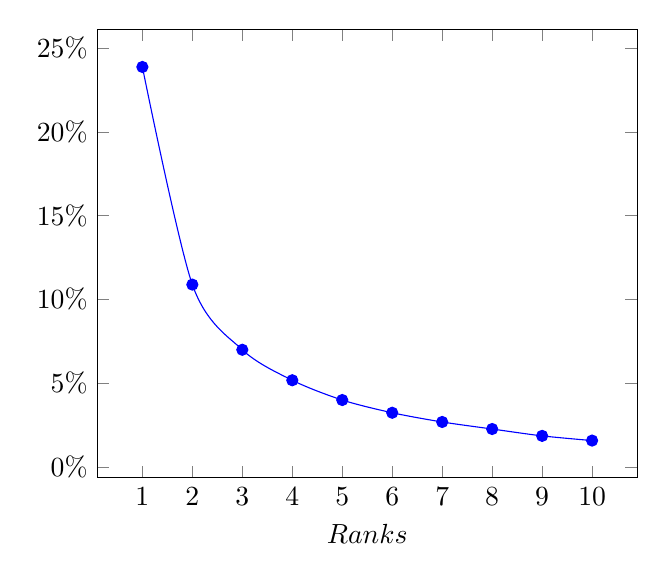
\begin{tikzpicture}
    \begin{axis}[
        xlabel=$Ranks$,
        %xmin=1,ymin=10,
        %ymin=0,
        %ymax=0.25]
        xtick={1,2,3,4,5,6,7,8,9,10},
        yticklabel={\pgfmathparse{\tick}\pgfmathprintnumber{\pgfmathresult}\%}]
    \addplot[smooth,mark=*,blue] plot coordinates {
        (1,23.87)
        (2,10.88)
        (3,6.99)
        (4, 5.17)
        (5, 3.99)
        (6, 3.23)
        (7, 2.68)
        (8, 2.26)
        (9, 1.85)
        (10, 1.57)
    };
    %\addlegendentry{Case 1}
    % \addlegendentry{Case 2}
    \end{axis}
    \end{tikzpicture}
    }
    \caption{Primary response frequency (in percent) versus rank for the Standard word list.}
    \label{fig:zipfianPlot}
\end{figure}
% \begin{figure}
% \centering
% \begin{tikzpicture}
% <code>
% \end{tikzpicture}
% \caption{M1} \label{fig:M1}
% \end{figure}

%\subsection{Stimulus Words}
%Next, we select the stimulus words by applying our previous experiments with nationality \cite{Garimella16} to India versus United States, and also extending it to gender for male versus female.
%Specifically, we select top 100 words from experiments for each demographic, which have the highest Adaboost accuracies over the baselines, and call them the \textit{culture} words and \textit{gender} words respectively.
%In addition to the 200 words selected in the above manner, we use the 100 association words as proposed by Kent and Rosanoff \shortcite{Kent10}, to form a total of 300 stimulus words.
%For each of these words, we collect response data to evaluate against from AMT, as described below.

%We conducted a word association survey on Mechanical Turk for participants from India and United States.
%This survey has two parts in it -- in the first part, the stimulus words were listed, and the respondents were asked to provide the first word they thought of when they saw the given stimulus word. 
%The second part of the survey contains demographic questions querying about gender, age, nationality, occupation, education level, income, etc. of the respondents.
%\FIXME{Include about spam detection?}.

%We conducted the above described AMT task for the 300 stimulus words twice, first with the constraint that the participants belong to United States, and the second with participants belonging to India.
%In each such survey, we seek for 400 HITs which approximate to 400 participants in the word association prediction (after removing spam respondents which are in the range of 10-40).


\paragraph {Analyses of Demographic Variations.} To model norm strength within a given demographic group or across groups, we tabulate how often respondents from a group match the most frequent answer ({\it Primary}) or one of the most frequent ten answers for that group ({\it Top10}). That is, given the response for one stimulus word as provided by one held-out survey respondent at a time, we determine whether that response matches the most frequent association of the {\it remaining} members of the same group %(i.e. excluding the held-out respondent)
(Table \ref{tab:intra-groupSimilarity}, {\it Primary} columns), or one of the top 10 associations pertaining to that same group
%, again removing the held-out respondent
(Table \ref{tab:intra-groupSimilarity}, {\it Top10} columns). Similarly, we measure the match with the most frequent or the top 10 responses from the other group, as shown in Table \ref{tab:inter-groupSimilarity}. As expected, the intra-group similarities are significantly higher than the inter-group similarities, which supports our hypothesis that different groups make different word associations, which tend to be more coherent within a group than across groups. While males and females have similar ranges for their agreement figures, we notice that on average US respondents have stronger intra-group agreements. Note also that inter-group similarities are asymmetrical, as multiple words may have the same association frequency for one group, yet for the complementary group that may not be the case.

As an additional analysis of demographic variations in the responses received, for each respondent, we predict his / her demographic group using a majority vote conducted across all the user's responses using a simple rule-based system that assigns each response to the group having the highest frequency for that particular association. For instance, given the response {\it sun} obtained from a respondent for the stimulus {\it yellow}, we assign the respondent to either India or US depending on the highest normalized frequency of the response {\it sun} for the same stimulus in each of those groups. 
A similar rule-based assignment is also used for gender. Thus, we compute the response words and their normalized frequencies based on the responses from $80\%$ of the users chosen randomly, and accordingly predict the demographic group for the remaining 20\% of the users based on a decision across the entire set of a user's responses. 
%to responses of the remaining $20\%$ of the users to predict their demographic groups.
 Table \ref{tab:eval3} shows the results of these predictions, which indicate high location variability (i.e., we can predict with high accuracy the location of a respondent), and medium gender variability. 

%To see how similar or different the associations of users belonging to each demographic value will be, we do the following -- for each user belonging to a nation (gender), check for each stimulus word if his/her response is the best association for that nation (gender) by assigning 1 for the best association and 0 otherwise. 
%Similarly, for each user, check if his/her answer falls in the top ten associations for that nation (gender) for each stimulus word and assign 1 in case of a match and 0 otherwise.
%The average best and out-of-ten (oot) scores across all the users for each stimulus word for each nation (gender) signify the intra-demographic similarity among users with respect to that word in the given demographic.



\begin{table}[ht]
\centering
\scalebox{0.85}{
\renewcommand{\arraystretch}{1}
\begin{tabular}{p{2.4cm}|c|c||c|c}
\hline
 Demo- & \multicolumn{2}{c||}{Standard} & \multicolumn{2}{c}{All} \\   
\cline{2-3} \cline{4-5}
graphic & Primary & Top10 & Primary & Top10 \\
\hline
\hline
India-India & 0.23 & 0.77 & 0.18 & 0.78\\
 US-US & 0.29 & 0.82 & 0.25 & 0.81\\
 Male-Male & 0.23 & 0.79 & 0.19 & 0.79 \\
 Female-Female & 0.25 & 0.80 & 0.21 & 0.81\\
\hline 
%Male & 2,031 & 597,935 \\
%Female & 1,818 & 321,779\\
%\hline
\end{tabular}
}
\caption{Intra-group similarities (the higher the similarity, the more cohesive the group is).}
\label{tab:intra-groupSimilarity}
\end{table}



\begin{table}[ht]
\centering
\scalebox{0.85}{
\renewcommand{\arraystretch}{1}
\begin{tabular}{p{2.4cm}|c|c||c|c}
\hline
 Demo- & \multicolumn{2}{c||}{Standard} & \multicolumn{2}{c}{All}  \\   
\cline{2-3} \cline{4-5}
graphic & Primary & Top10 & Primary & Top10 \\
\hline
\hline
India-US & 0.18 & 0.55 & 0.14 & 0.50\\
 US-India & 0.20 & 0.60 & 0.16 & 0.56\\
 Male-Female & 0.22 & 0.63 & 0.17 & 0.59 \\
 Female-Male & 0.24 & 0.66 & 0.19 & 0.61\\
\hline 
%Male & 2,031 & 597,935 \\
%Female & 1,818 & 321,779\\
%\hline
\end{tabular}
}
\caption{Inter-group similarities (the higher the similarity, the less distinct the groups are).}
\label{tab:inter-groupSimilarity}
\end{table}


\begin{table}[h]
\centering
\scalebox{0.85}{
\renewcommand{\arraystretch}{1}
\begin{tabular}{p{2cm}|c|c}
\hline
 Demographic & \multicolumn{1}{c|}{Standard} & \multicolumn{1}{c}{All} \\   
%\cline{2-3} \cline{4-5} \cline{6-7}
%graphic & best & oot & best & oot & best & oot \\
\hline
\hline
Gender & 0.60 & 0.56\\
 Location & 0.94 & 0.94\\
\hline 
%Male & 2,031 & 597,935 \\
%Female & 1,818 & 321,779\\
%\hline
\end{tabular}
}
\caption{Predictions based on similarity to group.}
\label{tab:eval3}
\end{table}

%Carmen: not sure if this is adding something of particular importance.
\begin{comment}
\begin{table}[ht]
\centering
\scalebox{0.95}{
\renewcommand{\arraystretch}{1}
\begin{tabular}{p{1cm}|c|c|c||c|c|c}
\hline
 Demo- & \multicolumn{3}{c||}{Standard} & \multicolumn{3}{c}{All}\\   
\cline{2-4} \cline{5-7}
graphic & 1 & 2 & 3 & 1 & 2 & 3\\
\hline
\hline
India & 0.24 & 0.12 & 0.08 & 0.19 & 0.10 & 0.07 \\
 US & 0.30 & 0.12 & 0.08 & 0.26 & 0.12 & 0.08\\
 Male & 0.25 & 0.11 & 0.08 & 0.21 & 0.10 & 0.08 \\
 Female & 0.26 & 0.12 & 0.08 & 0.22 & 0.11 & 0.08\\
\hline 
%Male & 2,031 & 597,935 \\
%Female & 1,818 & 321,779\\
%\hline
\end{tabular}
}
\caption{Percentage of users with the most popular, second most popular, and third most popular responses, averaged across the 100 standard stimulus words and all the 286 stimulus words.}
\label{tab:popularResponses}
\end{table}
\end{comment}


\section{Computational Models of Word Associations}
\label{models}
We first introduce a new model for measuring word associations that  leverages a shallow neural net architecture to embed demographically-enriched words. We then compare the performance of the predicted associations to those resulting from other approaches, including traditional corpus-based measures such as mutual information or vector-space models, as well as a recent distributed learning model with word embeddings. For each of these methods, we predict, evaluate, and compare generic associations (devoid of any demographic information), as well as demographic-aware associations.

%Then we also compare several other potential models, ranging from computationally simple (MI), to vectorial space models (VSMs), and a distributed learning model. All of these are employed first in a generic version, that is demographic-blind and which constitutes a baseline for each model, and then in a demographic-focused version, where each model attempts to encode word usage given demographic dimensions.

\subsection{Composite Skip-gram Models}
%still working on this section
We introduce a new word association model, which relies on the skip-gram neural net architecture \cite{Mikolov2013a}, and leverages its efficiency and  ability to deal with less frequent words. 

The skip-gram model tries to predict the context given a word, that is, for each word $w_i$ in the input sequence $w_1,\ldots,w_T$, the model tries to predict  $w_{i-2}$, $w_{i-1}$, $w_{i+1}$ and $w_{i+2}$, assuming, for example, a sliding window of five words. Mathematically, the model maximizes the objective function
\vspace{-0.5cm}
\begin{equation}
    J = \frac{1}{T}\sum_{i=1}^T\sum_{    j=-c, j\neq 0}^c \log P(w_{i+j}|w_i)
\end{equation}
%\vspace{-0.3cm}
\noindent where $T$ is the number of tokens in the data set, $c$ is the number of context words on each side of the target word $w_i$ and $P(w_{i+j}|w_i)$ is the probability to observe word $w_{i+j}$ in the context of word $w_i$.
%This method essentially allows generating a virtually unlimited number of training samples from plain text, being able to amplify the signature of $w_i$.

\begin{comment}
\begin{quote}
If your baby prefers warm formula or milk place a filled bottle in a bowl of warm water and let it stand for a few minutes.
\end{quote}
\end{comment}

To make this model demographic-aware, we propose two variations, which we refer to as composite skip-gram models ($C-SGM$). In the first one ($EMB1$), the target word $w_i$ is tagged with a demographic label $L$ (e.g., gender). For example, for the target word ``formula$^{L=\text{female}}$'' we try to predict a high probability for ``baby'' and ``milk'' occurring in the neighboring context. The underlying reasoning is that tagged words that appear in similar contexts will be nudged toward each other, while those that do not, will further distance themselves. This allows discrepancies to emerge between how the words are embedded given a demographic dimension. 

In the second variation ($EMB2$), we also include the demographic label in the context. That is, for each skip-gram $(c_{i,\text{left}}, w_i, c_{i,\text{right}})$ we generate three skip-grams
\vskip -0.2in
\begin{align}
&(c_{i,\text{left}}^{\text{label}}, \quad w_i, \quad c_{i,\text{right}})\nonumber\\ &(c_{i,\text{left}}, \quad w_i^{\text{label}}, \quad c_{i,\text{right}})\nonumber\\
&(c_{i,\text{left}}, \quad w_i, \quad c_{i,\text{right}}^{\text{label}})
\end{align}

The two models seek to capture different scenarios. In the first model, where we only add the demographic label to the target word, the embedding of the labeled word is optimized with respect to the generic embedding of the context. In the second model, the optimization is rather symmetric, allowing tagged and generic embeddings to influence each other. 
% NEW -- APARNA
Thus, the optimization function seeks to predict both tagged and untagged words in the vicinity given a target word, instead of only focusing on predicting untagged words like EMB1. The embeddings resulting from such a model should allow for more accurate representations across the tagged and untagged vocabulary, where for example the word ``mother'' uttered by a female would be close to the word ``mother'' (regardless of author gender).
% NEW -- APARNA
In both scenarios, the embeddings space accommodates both tagged and untagged words at the same time, being very computationally robust, and allowing comparisons across the tagged version of words, as well as between generic words and their tagged surrogates. For both variations, we compute the cosine similarity between the stimulus word and each of the vocabulary words (whether generic or demographic-enhanced), and retain the closest unique candidates (after dropping their demographic tag). 

%We train this model on a corpus enhanced with meta data information pertaining to the gender or culture of the authors. Each context is split into a 11 words window consisting of the target word in the center enhanced with the demographic dimension of the writer and 5 words to its left and right. The model is trained over these contexts, allowing demographic-enhanced words to coexist in the same latent dimension space with generic words; we will refer to this variation as {\it 1 section enhanced}. In order to provide additional data for demographic-aware embeddings to be learned, we train another model on the same contexts as before, yet each 11 word window is split into 3 sections, the target word, the left, and the right. Each context is represented 3 times, with each of the three sections appended at a time with demographic information, while the remaining sections are left in their generic forms. We will call this representation {\it 3 sections enhanced}. For both variations, we compute the cosine similarity between the stimulus word and each of the vocabulary words (whether generic or demographic-enhanced), and retain the closest unique candidates (after dropping their demographic annotation). 

\subsection{Other Word Association Models}


%tagged  using demographic information and without using demographic information, to test our hypothesis that knowledge of users' demographics can help better predict their word associations.
\paragraph{Mutual Information (MI).}
We implement the information theoretic measure proposed by Church and Hill \shortcite{Church90}.
It is defined as follows:
\begin{equation}
I(x, y) = log_{2}\frac{P(x, y)}{P(x)P(y)}
\end{equation}
This measure compares the probability of observing words $x$ and $y$ together (the joint probability) with the probabilities of observing $x$ and $y$ independently. 
%In this work, $x$ and $y$ represent words, and the word probabilities $P(x)$ and $P(y)$ are estimated by the frequencies of $x$ and $y$ in a corpus, $f(x)$ and $f(y)$, and normalizing by $N$, the size of the corpus.  
The joint probability, $P(x, y)$, is generally estimated by counting the number of times $x$ is followed by $y$ in a window of $w$ words, and normalizing this count with the size of the corpus. 
%Small window sizes can identify short range relations and fixed expressions (such as \textit{drink and drive}), while large window sizes can identify long range relations and semantic concepts. 
We follow Church and Hill and set the window size $w$ to five, as it is large enough to capture verb-argument constraints, and not so large to restrict to strict adjacency. 
For a given stimulus word, (1) we use the entire corpus and compute the generic MI word association with the rest of the vocabulary, and get the top associations according to their MI scores; and (2) we use the section of the corpus obtained for a given demographic, and determine the top  demographic-aware MI word associations. 

\paragraph{Vector-Space Model (VSM).}
% NEW -- APARNA
We also implement the traditional vector-space model, where each word is represented by a $tf.idf$ weighted vector inside the term-document matrix (representing term occurrences inside the documents in the corpus), with a length equal to the number of documents $D$ in the corpus \cite{Salton1986}. %, and each entry in these vectors representing the frequency of the word in the corresponding document divided by its document frequency acroand each word is represented in terms of the product of its frequency and inverse document frequency in each of the documents \cite{Salton1986}.
%Word vectors are constructed for all the words in the corpus.
% NEW -- APARNA
For a given stimulus word, cosine similarities are computed with all the remaining word vectors in the vocabulary, and those words having the highest similarity are considered as the top responses. 
Similar to MI, we use all the documents in the corpus to produce generic word associations, while only those documents pertaining to a specific demographic value are utilized to derive demographic-aware associations.  

\paragraph{Skip-gram Language Model.}
We also use the distributional representation technique of word embeddings ($SGLM$) proposed by Bamman et al. \shortcite{Bamman2014}.
Specifically, information about the speaker (geography, in their case) is used while learning the vector-space representations of word meanings from textual data that is supplemented with metadata about the authors.
In addition to the \textit{global} embedding matrix $W_{main}$ that contains low-dimensional representations for every word in the vocabulary \cite{Mikolov2013a}, this approach has an additional $|C|$ matrices $\{W_{c}\}$ of the same size as $W_{main}$, where $|C|$ denotes the number of values the demographic variable has in the data (e.g., if gender is the demographic variable, $C = \{female, male\}$ and $|C| = 2$). 
Each of these $|C|$ matrices captures the effect that each demographic variable value has on each word in the vocabulary. 
To index the embedding of a stimulus word $w \in \mathbb{R}^{|V|\times k}$, the hidden layer $h$ is computed as the sum of the matrix multiplications with each of the independent embeddings:
\vskip -0.2in
\begin{equation}
h = w^{T}W_{main} + \Sigma_{c \in C}w^{T}W_{c}
\label{eq:hiddenlayer}
\end{equation}
It then predicts the value of the context word $y$ using another parameter matrix $X \in \mathbb{R}^{|V|\times k}$ based on a softmax function $o = softmax(Xh)$, where $o \in \mathbb{R}^{|V|\times k}$.
Backpropagation using (input $x$, output $y$) word tuples learns the values of the various embedding matrices $W$ and parameter matrix $X$, which maximize the likelihood of context words $y$ conditioned on the stimulus word $x$.
%This approach is proposed and described in detail in the original paper \cite{Bamman2014}.

We use this approach in its original implementation provided by \cite{Bamman2014} to compute the word embedding vectors for all the words in the vocabulary.
Given a stimulus word, the closest vocabulary words with the highest cosine similarity are retained as the top association predictions for the given stimulus word.


\section{Experiments}
All our models require textual data with demographic information. We introduce below the data we used and the metrics we adopted for evaluation.

\paragraph{Data.}
Given the requirement of having gender and location information associated with the data, we resort to blogs, and collect from Google Blogger\footnote{\url{www.blogger.com}} a large set of blog posts  authored between 1999 and 2016. \tabref{tab:blogStats} shows the breakdown of the raw blog counts per demographic category. From these, we retain only those posts with non-empty content, and preprocess the data by removing HTML tags, converting all the tokens to their lemmatized forms,\footnote{We normalize the word forms using the Stanford CoreNLP lemmatizer \cite{Manning14}.} and discarding those lemmas with a frequency less than 10, in order to avoid misspellings and other noise characteristic to social media content.


\begin{table}[ht]
\centering
\scalebox{0.8}{
\renewcommand{\arraystretch}{1.05}
\begin{tabular}{p{1cm}|c|c|c|c|c}
\hline
%& \multicolumn{2}{c}{Male} & \multicolumn{2}{c}{Female}
%\cline{2-4} \cline{4-5}
\multirow{2}{1cm}{Demo-graphic} & \multicolumn{2}{c|}{Raw} &  \multicolumn{3}{c}{Balanced}\\
\cline{2-6}
 & Profiles & Posts & Profiles & Posts & Tokens\\
\hline
\hline
India & 1,520 & 339,624  & 1,520 & 34,987 & 16,884K\\
US & 3,273 & 825,093 & 1,520 & 32,782 & 11,706K \\
\hline 
Male & 2,031 & 597,935 & 1,818 & 44,299 & 21,971K\\ 
Female & 1,818 & 321,779 & 1,818 & 45,980 & 17,070K\\
\hline
\end{tabular}
}
\caption{Raw and balanced blog dataset statistics.}
\label{tab:blogStats}
\end{table}


%\subsection{Data for Association Predictions}
From the above pool of blog posts, we create two datasets with complementary demographic classes (1) location: India-US and (2) gender: male-female. %, as well as a third data set with four classes -- (3) quarters: India female - India male - US female - US male.

We process each of these datasets so that they are profile-balanced with no peaks for any specific years, by applying several heuristics:
%\footnote{The exact details for balancing the data are described in an addendum available at \url{http://lit.eecs.umich.edu/downloads.html}.}.
% END NEW -- APARNA
%CB: I think this information is too technical and is more suited for the readme file.
\textbf{(1)} Compute the minimum number of users $n$ over all the classes (e.g., Indian and US authors in the case of the location dataset). \textbf{(2)} From each class, select the top $n$ users based on the number of years they were blogging and the number of posts they wrote.\footnote{Prolific users will be chosen first. For a class with exactly $n$ users, all users will be chosen.} This ensures that the maximum amount of data will be available for the selected users. \textbf{(3)} For each of these $n$ users, pick at most 50 posts in a round-robin fashion from the years in which they blogged. \textbf{(4)} Let $M$ be the total number of posts collected in this manner from all the classes. In order to avoid having most of the posts coming from a small number of years, set a cutoff $X$ as a fraction of $M$. For each year, a maximum of $X$ posts will be chosen from the set of $M$ posts ($X = 0.1M$). \textbf{(5)} To ensure that all the users get to contribute posts, and that the contribution of prolific writers is kept in check, maintain user participation scores: 
\vskip -0.3in
    \begin{equation}
    p(user) = \textfrac{posts collected from user}{total number of posts collected}
    \end{equation}
\vskip -0.1in
\noindent These scores are updated after every year is processed, as explained further. % data from a given year is added to the corresponding data set. 
    \textbf{(6)} Sort the years in increasing order of number of posts and iterate through them; identify the lowest number of posts contributed by the least prolific writer, then collect the minimum number of posts from all users who published in that year in a round-robin manner. Then, select additional posts from users in increasing order of participation scores, until the number of posts for the year reaches the cutoff $X$. \textbf{(7)} After each year, update the user participation scores.
\tabref{tab:blogStats} shows the number of users and posts retained after balancing. This particular composition is used in our {\it location} data set (consisting of India and US posts) and {\it gender} data set (consisting of females and males posts). %We also compile two {\it generic} datasets, by combining the two location datasets, or the two gender datasets. %We further refine a third {\it quarters} dataset (with four demographic classes, 16M tokens), such that the number of authors in each quarter is the same, allowing us to make more accurate direct comparisons across evaluations, given the standardized data set composition. 


\begin{comment}
\begin{table}[ht]
\centering
\scalebox{0.9}{
\renewcommand{\arraystretch}{1.05}
\begin{tabular}{p{1.5cm}|c|c|c}
\hline
%& \multicolumn{2}{c}{Male} & \multicolumn{2}{c}{Female}
%\cline{2-4} \cline{4-5}
Data    & Profiles & Posts & Tokens\\
\hline
\hline
\multicolumn{4}{c}{Location}\\
\hline
India & 1,520 & 34,987 & \\
US & 1,520 & 32,782 & \\
\hline
\hline
\multicolumn{4}{c}{Gender}\\
\hline 
Male & 1,818 & 44,299 & \\ 
Female & 1,818 & 45,980 &\\
\hline
\end{tabular}
}
\caption{Blog statistics.}
\label{tab:datasetStats}
\end{table}
\end{comment}



\begin{comment}
\begin{table}[ht]
\centering
\scalebox{0.9}{
\renewcommand{\arraystretch}{1.05}
\begin{tabular}{p{1.8cm}|c|c|c|c}
\hline
%& \multicolumn{2}{c}{Male} & \multicolumn{2}{c}{Female}
%\cline{2-4} \cline{4-5}
Dataset & Users$_{1}$ & Posts$_{1}$ & Users$_{2}$ & Posts$_{2}$\\
\hline
\hline
location & 1,520 & 34,987 & 1,520 & 32,782 \\
\hline
gender & 1,818 & 44,299 & 1,818 & 45,980 \\
\hline
%quarters&&&\\
%~~~location & 656 & 12,286 & 656 & 19,972 \\
%~~~gender & 656 & 11,605 & 656 & 20,653 \\
%\hline
\end{tabular}
}
\caption{User and post counts for each class in various datasets (class$_{1}$-class$_{2}$).}
\label{tab:datasetStats}
\end{table}
%Two datasets: super-balanced one; very large gender or very large culture data
\end{comment}


\paragraph{Metrics.}
Given that the word association task is relatively similar to the lexical substitution task, in terms of open vocabulary and lack of a ``right'' answer, we decided to borrow the {\it best} and out-of-ten ({\it oo10}) evaluation metrics traditionally used for the latter \cite{McCarthy2009}, yet corrected for weight \cite{Jabbari2010}. Briefly, these measures take the best (or top ten) responses from a system, and compare them against  the gold standard, while accounting for the frequencies of the responses in the gold standard. In addition, since \figref{fig:zipfianPlot} shows that the top three ranking norms are provided as answers by approximately 42\% of the respondents, with the remaining norms following a long Zipfian distribution in terms of frequency of appearance, we also compute out-of-three ({\it oo3}), which represents a more focused approximation of our ability to predict human associations (note that out-of-ten covers 62\% of the responses).
 Several recent papers on word associations evaluated their models indirectly via Pearson or Spearman correlation performance on a word similarity task \cite{Chaudhari11,Deyne16}; we choose instead to evaluate word associations directly, by using metrics that more closely align with the evaluations performed in the field of psychology where the best output of a system is compared against the most frequent human response \cite{Bel14,Mohammad11}.


For a given stimulus word $w$ with human responses $H_{w}$, suppose a system returns a set of answers $S_{w}$. 
We estimate how well this system can find a \textit{best} substitute for $w$ using Equation \ref{eq:best}, where the function $freq_{w}(s)$ returns the count of a system response $s$ in $H_{w}$, and $maxfreq_{w}$ returns the maximum count of any response in $H_{w}$.
\begin{equation}
    best(w) = \frac{\Sigma_{s \in S_{w}}freq_{w}(s)}{maxfreq_{w} \times |S_{w}|}
    \label{eq:best}
\end{equation}
\begin{equation}
    oo\textbf{n}(w) = \frac{\Sigma_{s \in S_{w}^{n}}freq_{w}(s)}{|H_{w}|}
    \label{eq:oon}
\end{equation}
Equation \ref{eq:oon} measures the coverage of a system by allowing it to offer a set $S_{w}^{n}$ of \textit{n} responses for $w$, where each response $s$ is weighted by its frequency $freq_{w}(s)$ in $H_{w}$.


%TODO-CB-NEW the paragraph below is what I had earlier, but I think that your answer covers this. We can comment it out.
%While rank correlation is the de facto evaluation metric for word similarity and relatedness, the task of word association is different, as all the primary answers given by respondents are considered correct. A given answer cannot be directly compared with another, and a ranking only emerges upon considering all responses for a given word. As such, while for word similarity, the similarity score for a given pair $a$ and $b$ represents how semantically related the tokens are, and the scoring allows for similarity comparison with another word pair, for word association this is not the case, and the ranking can only exist in regards to the responses provided for the stimulus word.


\section{Evaluations and Discussions}

\begin{table*}[ht!]
\centering
\scalebox{0.9}{
\begin{tabular}{l|l||c|c||c|c||c|c||c|c||c|c||c|c}
\hline
	&		&	\multicolumn{2}{c||}{best}			&	\multicolumn{2}{c||}{oo3}			&	\multicolumn{2}{c||}{oo10}			&	\multicolumn{2}{c||}{best}			&	\multicolumn{2}{c||}{oo3}			&	\multicolumn{2}{c}{oo10}			\\
	\cline{3-14}																							
Method	&	Type	&	IN	&	US	&	IN	&	US	&	IN	&	US	&	M	&	F	&	M	&	F	&	M	&	F	\\
\hline	\hline										
%GS	&		&	0.58	&	0.58	&	0.74	&	0.77	&	0.82	&	0.86	&	0.77	&	0.76	&	0.82	&	0.84	&	0.84	&	0.88	\\
%\hline
MI	&	Gen	&	0.00	&	0.00	&	0.01	&	0.01	&	0.02	&	0.01	&	0.01	&	0.01	&	0.01	&	0.01	&	0.01	&	0.01	\\
	&	DA	&	0.00	&	0.00	&	0.01	&	0.00	&	0.02	&	0.02	&	0.00	&	0.01	&	0.01	&	0.01	&	0.01	&	0.02	\\
\hline
VSM	&	Gen	&	0.00	&	0.00	&	0.01	&	0.01	&	0.03	&	0.03	&	0.00	&	0.00	&	0.02	&	0.02	&	0.05	&	0.05	\\
	&	DA	&	0.00	&	0.00	&	0.02	&	0.01	&	0.04	&	0.02	&	0.00	&	0.01	&	0.02	&	0.01	&	0.04	&	0.06	\\
\hline
SGLM	&	Gen	&	0.02	&	0.02	&	0.03	&	0.03	&	0.06	&	0.05	&	\textbf{0.13}	&	0.13	&	\textbf{0.18}	&	{\it 0.18}	&	0.20	&	0.21	\\
	&	DA	&	0.05	&	0.01	&	0.07	&	0.02	&	0.11	&	0.03	&	0.10	&	0.13	&	0.16	&	{\it 0.18}	&	0.18	&	0.20	\\
\hline
\multirow{3}{2cm}{C-SGM}	&	Gen	&	0.05	&	\textbf{0.04}	&	0.07	&	\textbf{0.07}	&	0.11	&	\textbf{0.10}	&	{\it 0.11}	&	0.13	&	{\it 0.17}	&	0.17	&	0.20	&	0.21	\\
	&	EMB1	&	{\it 0.08}	&	{\it 0.03}	&	{\it 0.12}	&	\textbf{0.07}	&	{\it 0.18}	&	\textbf{0.10}	&	\textbf{0.13}	&	{\it 0.14}	&	\textbf{0.20}	&	\textbf{0.20}	&	\textbf{0.25}	&	\textbf{0.26}	\\
	&	EMB2	&	\textbf{0.09}	&	0.02	&	\textbf{0.14}	&	{\it 0.04}	&	\textbf{0.19}	&	{\it 0.06}	&	0.10	&	\textbf{0.16}	&	{\it 0.17}	&	\textbf{0.20}	&	{\it 0.23}	&	{\it 0.25}	\\
	\cline{2-14}
%	&	EMB1-unbal	&	\textbf{0.11}	&	\textbf{0.13}	&	\textbf{0.17}	&	\textbf{0.15}	&	\textbf{0.21}	&	\textbf{0.17}	&	0.09	&	\textbf{0.16}	&	0.17	&	0.18	&	0.21	&	0.23	\\
%	& unbal & & & & & & & & & & & & \\
	\hline
	\hline
\multirow{2}{2cm}{C-SGM-raw}	&	EMB1	&	0.11	&	0.13	&	0.17	&	0.15	&	0.21	&	0.17	&	0.09	&	0.16	&	0.17	&	0.18	&	0.21	&	0.23	\\
	&	EMB2	&	0.10	&	0.08	&	0.15	&	0.12	&	0.19	&	0.15	&	0.09	&	0.14	&	0.15	&	0.16	&	0.18	&	0.20	\\
	\cline{1-14}
\end{tabular}
}
\caption{Best, out-of-three (oo3), and out-of-ten (oo10) scores across the various methods. %GS: Gold Standard, 
IN: India, US: United States, M: Male, F: Female. The numbers in bold mark the highest scores, those in italics, the second highest.}
\label{tab:results}
\end{table*}


We conduct evaluations using all the word association models described in Section \ref{models}. The results using the {\it best}, {\it out-of-three}, and {\it out-of-ten} evaluation metrics are listed in Table \ref{tab:results}. For all the embeddings experiments, we use 300 latent dimensions. The $Gen$ variation uses the demographic-blind dataset, whereas the $DA$ variation  uses the demographic-aware dataset.\footnote{To place the results in this table in perspective, it is important to note that results for this task are traditionally low. Given that the most frequent response is selected on average by 24\% of respondents (see Figure \ref{fig:zipfianPlot}), we can see that even for humans, the highest score would be around 0.24.}  
%We also include an upper bound computed over the gold standard association norms, by considering the top ranking associations for a given group as gold standard, and the predictions of its complementary demographic group as system predictions, and then compute the same {\it best}, {\it out-of-three}, and {\it out-of-ten} evaluation scores.

The MI and VSM models do not perform well in the word association prediction task, whether considering the generic or the demographic-aware data. We should emphasize, however, that the generic version of these models is able to consider co-occurrences across the entire generic datasets, while the demographic-aware co-occurrences can only be computed from the section of the dataset that matches a particular demographic; as such, these latter models are placed at a disadvantage. 

Perhaps not surprisingly, the neural network skip-gram-based architectures, whether SGLM or our C-SGM, always achieve better results when compared to MI or VSM. The demographic-aware variation proposed by \cite{Bamman2014} uses an extended skip-gram architecture that encodes a generic embedding, and several demographic-based filters per class, which in our case translates into three matrices of 300 dimensions each, the first for the generic words, and the subsequent ones for skews to be applied to the generic words in order to render the embedding through the lens of a given demographic. $SGLM-Gen$ in our case are the predictions based on the generic matrix, while $SGLM-DA$ are the predictions modified along the lines of a particular demographic. 

Our composite skip-gram models encode a single matrix that contains a mix of demographic-aware and generic words expressed as 300 latent dimensions. For both gender and location, our gender-aware models ($EMB1$ and $EMB2$) surpass the SGLM gender-aware model. Surprisingly, while SGLM was never meant to be generic, the predictions based on its generic embedding matrix prove to be a difficult baseline to surpass, similar to C-SGM generic. Nonetheless, the composite skip-gram models ($EMB1$ and $EMB2$) do achieve best and second best rankings in the vast majority of cases (when compared to the best among all the other methods), with $EMB1$ being the more robust variation performing well both for gender and for location. % for gender, for the {\it best} metric, our models are able to achieve 0.14 - 0.16 for Female-focused embeddings (versus 0.13), and for Male, 0.09-0.10 versus 0.13; for out-of-three, for female, we achieve 0.2 (versus 0.18), and for male 0.17 (versus 0.18); for out-of-ten, for female we achieve between 0.25 and 0.26 (compared to 0.21), while for male we achieve between 0.21 and 0.23 (compared to 0.20). Similarly, for location, in best for India, we score 0.08 - 0.09 (compared to 0.05), while best for US, we score between 0.02-0.03 (versus 0.04); in out-of-three for India, we score 0.12 - 0.14 (versus 0.07), and for US, 0.04-0.07 (versus 0.07); in out-of-ten for India, we score between 0.18 and 0.19 versus 0.11, while for US, we score between 0.06 and 0.10 versus 0.10. 
Focusing on the performance of $EMB1$, the highest gains are observed for India-based predictions, for best (from 0.05 to 0.08) and out-of-three (from 0.07 to 0.12); for male-based predictions increasing from 0.11 to 0.13 for best, and from 0.17 to 0.20 for out-of-three; and for female-based predictions, increasing from 0.13 to 0.14 for best, and from 0.17 to 0.20 for out-of-three.  US-based associations are the hardest to predict, probably because of the diverse makeup of society; additional evaluations are needed to pinpoint the exact cause. 
%TODO-Rada-New -- I updated some numbers in the table above, they were not matching the table
%TODO-Carmen-New -- We updated the text to only reference EMB1, instead of picking the best results between EMB1 and EMB2

To determine how susceptible the embedding model is to skewed, but larger training data, we also run a separate experiment on the entire raw set of blogs we collected (described on the left of Table \ref{tab:blogStats}), where we re-generate the $EMB1$ and $EMB2$ models. While the entire dataset is significantly larger than the balanced set, it is also significantly skewed: 
%The results from this evaluation are shown in row $EMB1-unbal$ in  \tabref{tab:results}. 
the data in the India:US dataset was skewed in a proportion of 1:0.48 tokens, while for Female:Male the proportion was 1:0.41 tokens. As was the case for the balanced dataset, the $EMB1$ model is still the most robust (see the bottom section in Table \ref{tab:results}), and it achieves significant gains when compared to its balanced counterpart, in particular for {\it best} (for the US demographic from 0.03 to 0.13, and for India from 0.08 to 0.11), and for {\it out-of-three} (for US from 0.07 to 0.15, and for India from 0.12 to 0.17), which suggests that as an avenue for future research, we can explore the use of significantly larger even if unbalanced datasets to train our models. 

%\FIXME{One could question why not also train Bamman on the large unbalanced set. One way to try to counter-act that would be to list the EMB2 and EMB1-unbal variations in a separate table. Also why don't we use EMB2 for the unbalanced data?}
%Those evaluations are still running, as Bamman is very resource intensive and slow.
%We did include EMB2 results. We didn't have them ready before for the ACL deadline.

% precision: averages over words for which system gives non-empty responses; but our systems give non-empty responses to all the words; hence we just look at recall?




% \begin{table}[ht]
% \label{tab:results}
% \caption{\FIXME{Add oot results}}
% \end{table}[ht]


%precision-recall: precision at top 5 words, top 10 words, top 20, etc. Similarly recall;

%Compare with regular word associations with no profile -- (1) on a datset of comparable size with the profiles one; or (2) on larger data

%Comparison or discussion: look at previous results for the 100 words from the gray book (maybe just pick a few e.g., 5 words and see how our groups perform) 

\section{Conclusion}
In this paper, we introduced the task of demographic-aware word associations. To understand the various ways in which people associate words, we collected a new large demographics-enhanced dataset of approximately 300 stimulus words and their associated norms compiled from 800 respondents for a total of 176,097 non-spam responses, and show that for people of different demographics, associations do differ with gender and location. 
%We also show that conducting the task online via Amazon Mechanical Turk mirrors the results obtained using traditional word association surveys administered in classroom settings, providing additional backing to our data gathering method. 

We proposed a new demographic-aware word association method based on composite skip-gram models that are able to jointly embed generic and gender tagged words. We showed that this method improves over its generic counterpart, and also outperforms previously proposed models of word association, 
%%TODO-Rada-NEW
thus demonstrating that  it is useful to account for the demographics of the people behind the language when performing the task of automatic word association. We regard this as a first step toward demographic-aware NLP, and in future work we plan to address other more advanced NLP tasks while accounting for demographics. 

The word association dataset introduced in this paper is publicly available from \url{http://lit.eecs.umich.edu/downloads.html}. 
%further show that our models outperform not only traditional methods based on mutual information or VSM, but also demographics-aware language models (SGLM). %In addition, for Indian residents or for females, demographic-aware predictions are significantly better than the generic ones, providing support to the hypothesis that knowledge about the demographics of people can help in better predicting their word associations. %While for the United States we are unable to predict word associations successfully, we suspect this is caused by the significant heterogeneity of the population (and therefore of their association norms); however, additional studies are needed.
%\FIXME{mention about males?}
%Finally, we experiment our model with skewed data where we do not balance for the various demographic groups to see if balancing the data plays any role in predictions. This results in a significant increase in the association predictions in United States, highlighting the usefulness of large datasets in this kind of task.

\section*{Acknowledgements}
This material is based in part upon work supported by the Michigan Institute for Data Science, by the National Science Foundation (grant \#1344257), and by the John Templeton Foundation (grant \#48503). Any opinions, findings, and conclusions or recommendations expressed in this material are those of the author and do not necessarily reflect the views of the Michigan Institute for Data Science, the National Science Foundation, or the John Templeton Foundation. 


\bibliographystyle{emnlp_natbib}
\bibliography{aparna}
\end{document}